\documentclass[a4paper,12pt]{article}

\usepackage[top=2.5cm, bottom=2.5cm, left=3.175cm, right=3.175cm]{geometry}
\usepackage{polski}
\usepackage[utf8]{inputenc}
\usepackage{xcolor}
\usepackage{graphicx}
\usepackage{titlesec}
\usepackage{indentfirst}
\usepackage{amsmath}
\usepackage{float}
\usepackage{minted}
\usepackage[section]{placeins}
\usepackage{subfig}

% \usetikzlibrary{positioning}

\graphicspath{{images/}}

\numberwithin{equation}{section}

\newminted{cpp}{breaklines,linenos,frame=single}

\usepackage[pdftex,
            pdfauthor={Cezary Bober, Michał Kruczek},
            pdftitle={Dokumentacja projektu z przedmiotu Grafika Komputerowa},
            pdfsubject={Microcar Flex Furgon}]{hyperref}

\begin{document}

\pagenumbering{gobble}

\begin{titlepage}
    \includegraphics[height=1.75cm]{prz_pl.png}
    \hfill
    \includegraphics[height=1.75cm]{weii_pl.png}
    
    \centering
    \vfill
    
    {\Huge \textbf{Dokumentacja projektu z przedmiotu Grafika Komputerowa} \par}
	\vspace{1.5cm}
	{\LARGE Microcar Flex Furgon \par}
	
	\vfill
    
    {\Large \textbf{Cezary Bober} \par}
    {\Large \textbf{Michał Kruczek} \par}
    
    \vfill
    
    {\LARGE Rzeszów, 2019\par}
\end{titlepage}

\setlength{\parskip}{0.3cm}
\setlength{\parindent}{1cm}
\pagenumbering{arabic}
\setcounter{page}{2}

\tableofcontents
\pagebreak
%%%%%%%%%%%%%%%%%%%%%%%%%%%%%%%%%%%%%%%%%%%%%%%%%%%%%%%%%%%%%%%%%%%%%%%%%%%%%%%%%%%%%%%%%%%%%%%%%%%%%%%%%%

\section{Opis projektu}
Celem projektu było stworzenie interaktywnego modelu prostego samochodu korzystając z biblioteki OpenGL. Dzięki wykonaniu projektu poszerzyliśmy naszą wiedzę dotyczącą zarówno tworzenia modeli 3D jak i z pozostałych zagadnień składających się na dziedzinę jaką jest grafika komputerowa. 

Stworzony pojazd z pozwala na jazdę do przodu oraz do tyłu, zaimplementowane zostały także pewne elementy interaktywne takie jak otwieranie i zamykanie klapy bagażnika oraz maski. Samochód posiada także kręcący się wał napędowy napędzający potężny silnik.
%%%%%%%%%%%%%%%%%%%%%%%%%%%%%%%%%%%%%%%%%%%%%%%%%%%%%%%%%%%%%%%%%%%%%%%%%%%%%%%%%%%%%%%%%%%%%%%%%%%%%%%%%%

\subsection{Wykorzystane technologie}
Projekt został napisany przy wykorzystaniu języka C++ w wersji 11. Przy tworzeniu projektu wykorzystywaliśmy bibliotekę graficzną \textit{OpenGL}. Oprócz niej wykorzystana została biblioteka \textit{OpenGL Mathematics}, która pozwala na proste wykorzystanie bardziej skomplikowanych narzędzi aparatu matematycznego. Kolejną biblioteką była \textit{GLFW}, która zapewnia proste API do tworzenia okien, kontekstów i powierzchni, odbierania danych wejściowych i zdarzeń. Załadowanie tych bibliotek było możliwe dzięki bibliotece \textit{OpenGL Extension Wrangler Library}, która zapewnia wydajne mechanizmy uruchamiania w celu określenia, które rozszerzenia OpenGL są obsługiwane na platformie docelowej.

Modele poszczególnych części samochodu zostały stworrzone w narzędziu \textit{Blender}, który jest otwartym oprogramowaniem do modelowania i renderowania obrazów oraz animacji trójwymiarowych. Następnie dzięki bibliotece \textit{Open Asset Import Library} zostały one umieszczone w programie.

%%%%%%%%%%%%%%%%%%%%%%%%%%%%%%%%%%%%%%%%%%%%%%%%%%%%%%%%%%%%%%%%%%%%%%%%%%%%%%%%%%%%%%%%%%%%%%%%%%%%%%%%%%

\section{Inspiracja}
Inspiracją do stworzenia omawianego modelu samochodu był posiadany przez jednego z autorów projektu samochód \textit{Microcar MC1} przedstawiony na zdjęciu poniżej.
\begin{figure}[h!]
    \centering
    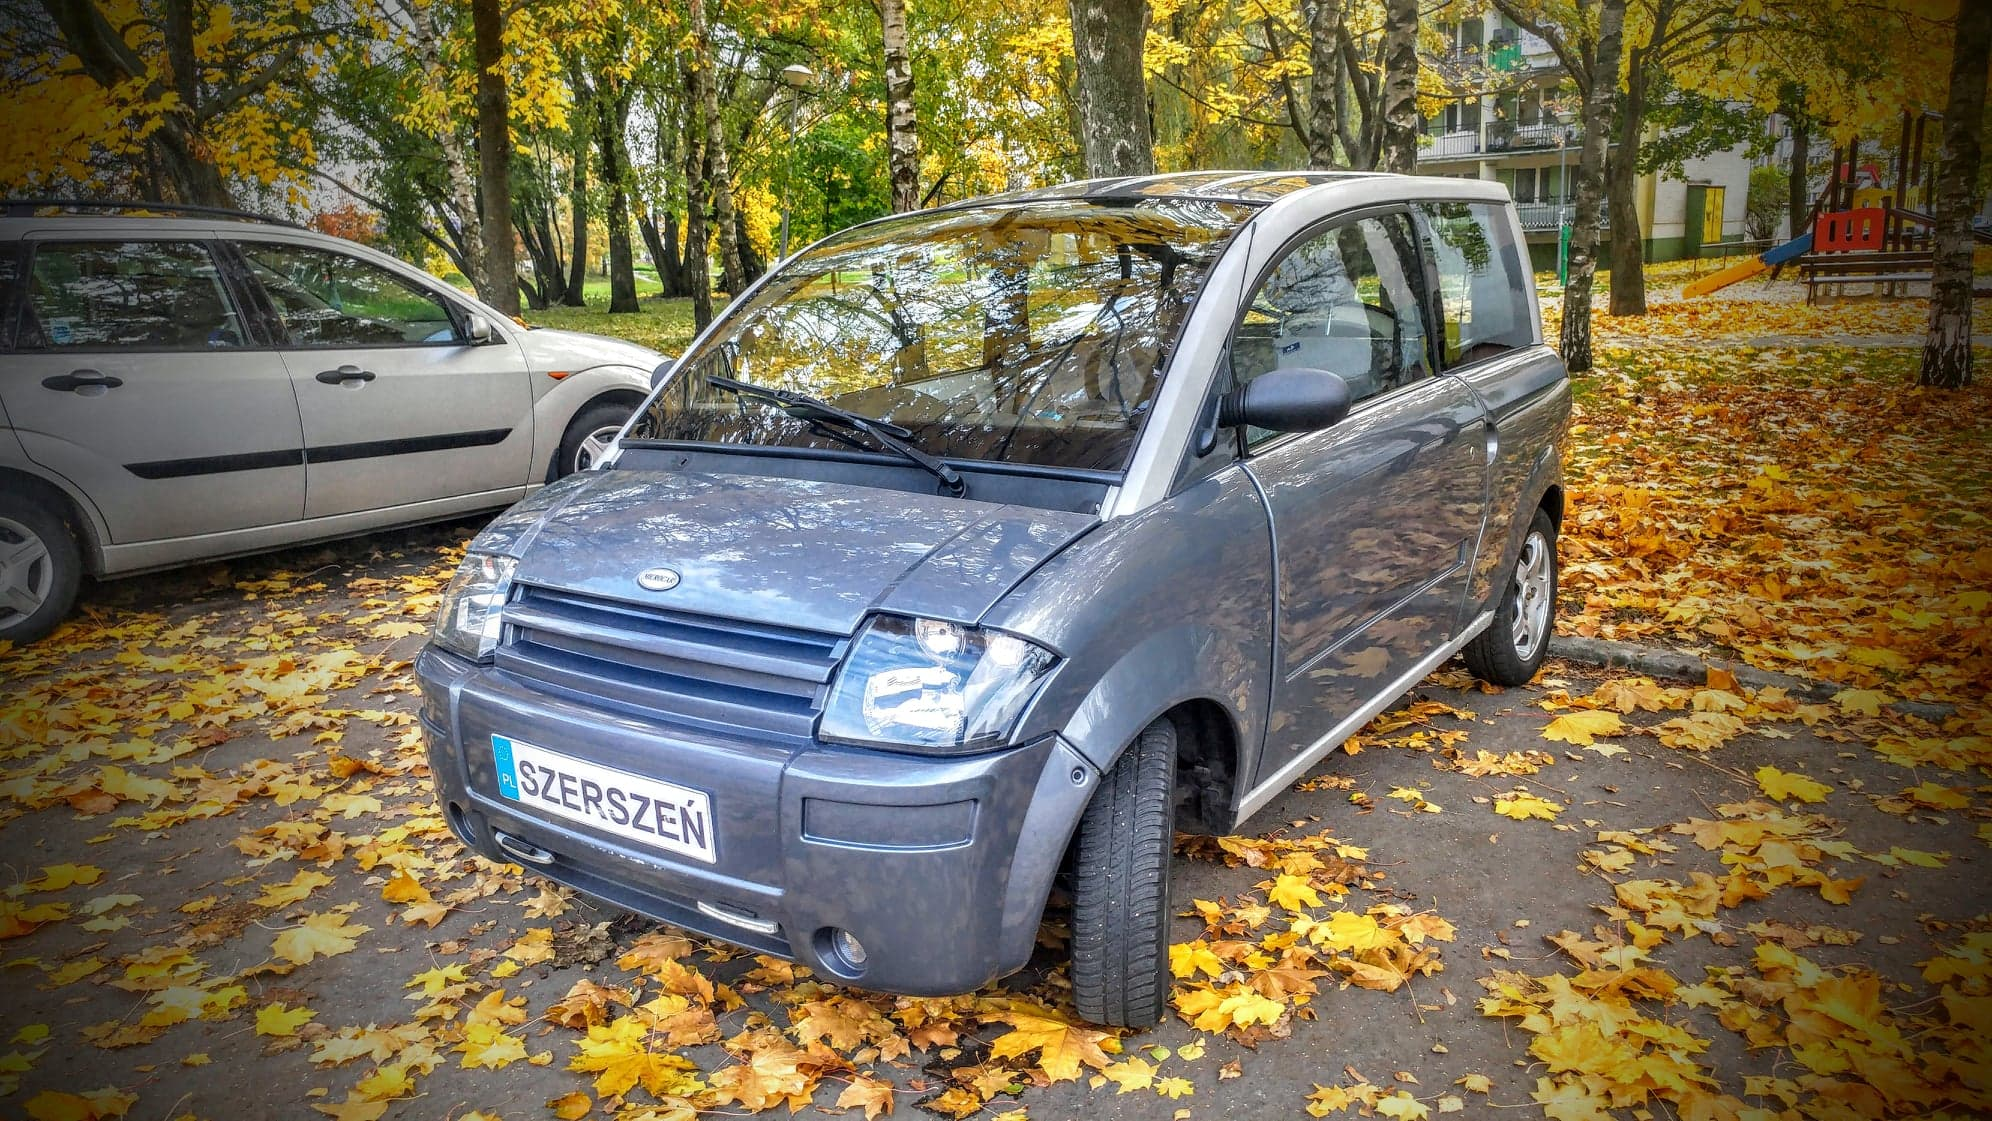
\includegraphics[width=\textwidth]{szerszen.jpg}
    \caption{Microcar MC1 \textit{"Szerszeń"}}
    \label{fig:szerszen}
    \vspace{1cm}
\end{figure}

Umieszczona w projekcie wersja jest modelem zmodyfikowanym na potrzeby handlu towarowego. Niewielkie rozmiary i mała waga powodują, że jest to bardzo dobry pojazd do ciasnych i zatłoczonych miast.
\begin{figure}[h!]
    \centering
    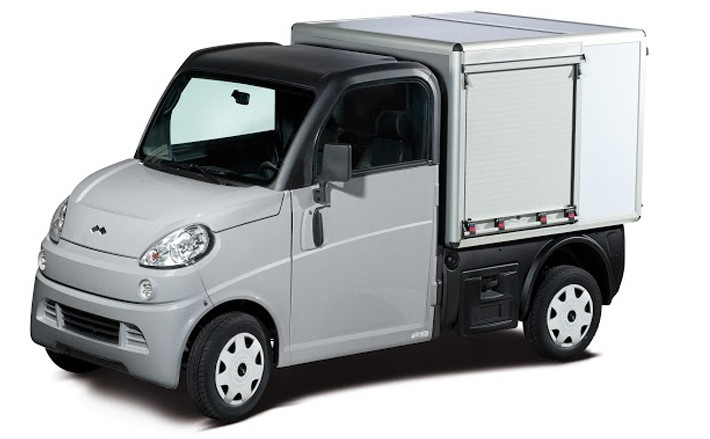
\includegraphics[width=0.8\textwidth]{furgon.jpg}
    \caption{Microcar Flex Furgon}
    \label{fig:furgon}
    % \vspace{0.5cm}
\end{figure}
%%%%%%%%%%%%%%%%%%%%%%%%%%%%%%%%%%%%%%%%%%%%%%%%%%%%%%%%%%%%%%%%%%%%%%%%%%%%%%%%%%%%%%%%%%%%%%%%%%%%%%%%%%

\section{Powstawanie projektu}
%%%%%%%%%%%%%%%%%%%%%%%%%%%%%%%%%%%%%%%%%%%%%%%%%%%%%%%%%%%%%%%%%%%%%%%%%%%%%%%%%%%%%%%%%%%%%%%%%%%%%%%%%%

\subsection{Plik główny}

\begin{center}
    Main.cpp
\end{center}

\begin{cppcode}
GLfloat deltaTime = 0.0f;
GLfloat lastTime = 0.0f;
GLfloat timeCounter = 0.0f;
int frameCount = 0;

static const char* vShader = "Shaders/shader.vert";
static const char* fShader = "Shaders/shader.frag";

void computeFPS(GLFWwindow* pWindow);

int main()
{
	Window mainWindow(1200, 800);
	mainWindow.Initialize();

	while (!mainWindow.getShouldClose())
	{
		computeFPS(mainWindow.mainWindow);

		glfwPollEvents();

		glClearColor(0.0f, 0.0f, 0.0f, 1.0f);
		glClear(GL_COLOR_BUFFER_BIT | GL_DEPTH_BUFFER_BIT);

		glUseProgram(0);
		mainWindow.swapBuffers();
	}

	return 0;
}
\end{cppcode}

Pierwszym plikiem jaki zostął stworzony podczas tworzenia programu był plik Main.cpp wraz z główną funkcją. Funkcja ta jest samym centrum programu. W pętli głównej będą wywoływane główne funkcje odpowiedzialne za obsługę zdarzeń, obsługę shaderów oraz renderowanie poszczególnych elementów.
To własnie ta pętla odpowiada za ponowne wyświetlanie wszystkich elementów.

\begin{cppcode}

void computeFPS(GLFWwindow* pWindow)
{
	GLfloat now = glfwGetTime();
	deltaTime = now - lastTime;
	lastTime = now;
	timeCounter += deltaTime;
	frameCount++;

	if (timeCounter >= 1.0) {
		double fps = double(frameCount) / timeCounter;

		std::stringstream ss;
		ss << " [" << fps << " FPS]";

		glfwSetWindowTitle(pWindow, ss.str().c_str());

		frameCount = 0;
		timeCounter = 0;
	}
}
\end{cppcode}

Pierwszą funkcje jaka została zainmplementowana w programie to był licznik kaltek na sekundę, który następnie został umieszczony w tytule okna. Dzięki niemu w łatwy sposób mogliśmy określić wydajność naszej aplikacji. Licznik ten działa w oparciu o ilość czasu który upłynął pomiędzy kolejnymi iteracjami programu.
\newline
\indent Aby uniknąć nadmiarowej ilośći kodu w głownym pliku aplikacji, całość kodu odpowiedzialnego za inicjalizacje oraz konfigurację okna został umieszczony w osobnym pliku o nazwie Window.cpp
\begin{cppcode}

int Window::Initialize()
{
	if (!glfwInit())
	{
		printf("Error Initialising GLFW");
		glfwTerminate();
		return 1;
	}

	glfwWindowHint(GLFW_CONTEXT_VERSION_MAJOR, 3);
	glfwWindowHint(GLFW_CONTEXT_VERSION_MINOR, 3);

	glfwWindowHint(GLFW_OPENGL_PROFILE, GLFW_OPENGL_CORE_PROFILE);

	glfwWindowHint(GLFW_OPENGL_FORWARD_COMPAT, GL_TRUE);

	glfwWindowHint(GLFW_REFRESH_RATE, 60);

	const GLFWvidmode* mode = glfwGetVideoMode(glfwGetPrimaryMonitor());
    glfwGetPrimaryMonitor(), NULL);
	mainWindow = glfwCreateWindow(width, height, "Microcar Flex Furgon", NULL, NULL);
	width = mode->width;
	height = mode->height;
	if (!mainWindow)
	{
		printf("Error creating GLFW window!");
		glfwTerminate();
		return 1;
	}

	glfwGetFramebufferSize(mainWindow, &bufferWidth, &bufferHeight);

	glfwMakeContextCurrent(mainWindow);

	createCallbacks();
	glfwSetInputMode(mainWindow, GLFW_CURSOR, GLFW_CURSOR_DISABLED);

	glewExperimental = GL_TRUE;

	GLenum error = glewInit();
	if (error != GLEW_OK)
	{
		printf("Error: %s", glewGetErrorString(error));
		glfwDestroyWindow(mainWindow);
		glfwTerminate();
		return 1;
	}

	glEnable(GL_DEPTH_TEST);

	glViewport(0, 0, bufferWidth, bufferHeight);

	glfwSetWindowUserPointer(mainWindow, this);
}
\end{cppcode}

W funkcji inicjalizacyjnej okna ustawiane są wszelkie niezbędne parametry do utworzenia okna aplikacji. Definiowany jest rozmiar okna, tryb pracy biblioteki openGl, a także odświeżanie okna oraz obsługa zdarzeń. W aplikacji została zainmplementowana obsługa zdarzeń, po przez stworzenie jednej wielkiej tablicy z aktualnym stanem klawiszy.
\newline

\indent W celu obsługi zdarzeń klawiszy została stworzona funkcja o nazwie handleKeys, która została przedstawiona w listingu kodu poniżej. W funkcji tej wykrywane jest, który klawisz został naciśnięty i odpowiednio zmieniany jest jego stan w tablicy.

\begin{cppcode}
void Window::handleKeys(GLFWwindow* window, int key, int code, int action, int mode)
{
	Window* theWindow = static_cast<Window*>(glfwGetWindowUserPointer(window));

	if (key == GLFW_KEY_ESCAPE && action == GLFW_PRESS)
	{
		glfwSetWindowShouldClose(window, GL_TRUE);
	}
	else if (key >= 0 && key < 1024)
	{
		if (key == GLFW_KEY_B && action == GLFW_PRESS)
		{
			theWindow->keys[key] = !theWindow->keys[key];
		}
		else if (key == GLFW_KEY_B && action == GLFW_RELEASE)
			return;
		else if (action == GLFW_PRESS)
		{
			theWindow->keys[key] = true;
		}
		else if (action == GLFW_RELEASE)
		{
			theWindow->keys[key] = false;
		}
	}
}
\end{cppcode}

W kolejnym listiningu code przedstawione jest to jak stworzona została funkcja przechwytująca ruchy myszką. Są one tak samo przechowywane w odpowiednich zmiennych, aby można było w łatwy sposób z nich korzystać.

\begin{cppcode}
    

void Window::handleMouse(GLFWwindow* window, double xPos, double yPos)
{
	Window* theWindow = static_cast<Window*>(glfwGetWindowUserPointer(window));

	if (theWindow->mouseFirstMoved)
	{
		theWindow->lastX = xPos;
		theWindow->lastY = yPos;
		theWindow->mouseFirstMoved = false;
	}

	theWindow->xChange = xPos - theWindow->lastX;
	theWindow->yChange = theWindow->lastY - yPos;

	theWindow->lastX = xPos;
	theWindow->lastY = yPos;
}

\end{cppcode}

W celu implementacji tych własnoręcznie napisanych funkcji obsługi zdarzeń, zostały one podpięte pod callbacki funkcji OpenGl'owych.

\begin{cppcode}

void Window::createCallbacks()
{
	glfwSetKeyCallback(mainWindow, handleKeys);
	glfwSetCursorPosCallback(mainWindow, handleMouse);
}

\end{cppcode}

Klasa Window, posiada również dwa konstruktory. Jeden z nich służy do utworzenia okna o zadanym rozmiarze, natomiast drugo tworzy okno o rozmiarze 800x600 [px]. Można znaleść również destruktor tej klasy który uwalnia pamięć, która była wykorzystywana przez ten obiekt. 

%%%%%%%%%%%%%%%%%%%%%%%%%%%%%%%%%%%%%%%%%%%%%%%%%%%%%%%%%%%%%%%%%%%%%%%%%%%%%%%%%%%%%%%%%%%%%%%%%%%%%%%%%%


\subsection{Kamera}
Aby móc modyfikować to co użytkownik widzi na ekranie napisana została klasa \mintinline{cpp}{Camera} implementująca kamerę. Aby zdefiniować kamerę, potrzebujemy jej pozycji w przestrzeni świata, kierunku, w którym patrzy, wektora wskazującego w prawo i wektora skierowanego w górę od kamery. Będziemy tworzyć układ współrzędnych z 3 prostopadłymi do siebie osiami jednostkowymi z pozycją kamery jako początkiem układu.

\begin{figure}[H]
    \centering
    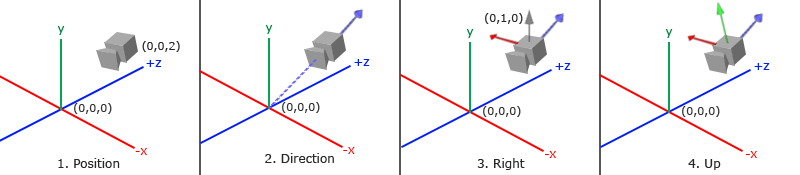
\includegraphics[width=\textwidth]{camera_axes.png}
    \caption{Najważniejsze parametry kamery}
    \label{fig:camera}
    % \vspace{0.5cm}
\end{figure}

Jeżeli zdefiniuje się przestrzeń współrzędnych za pomocą 3 prostopadłych (lub nie liniowych) osi, można utworzyć macierz z tymi 3 osiami i wektorem translacji, dzięki czemu można przekształcić dowolny wektor do tego stworzonego układu współrzędnych, mnożąc ten wektor przez tą macierz. Ta zależność znacznie ułatwia dalszą implementację kamery. Opisany wyżej proces jest realizowany przez funkcję \mintinline{cpp}{glm::lookAt()}, która wymaga wektora pozycji, punktu, na który ma być skierowana kamera i górnego wektora. Tworzy ona odpowiednią macierz widoku.

Kolejnym krokiem było umożliwienie poruszania kamerą przez użytkownika. W tym celu utworzona została funkcja \mintinline{cpp}{MouseControl()}, dzięki której każdorazowe naciśnięcie jednego z klawiszy strzałek spowoduje aktualizację pozycji kamery. Do poruszania się do przodu lub do tyłu, należy dodać lub odjąć wektor kierunku od wektora położenia. Natomiast do przesuwania się na boki, wykonać iloczyn wektorowy, aby utworzyć prawy wektor i odpowiednio poruszać się wzdłuż tego wektora w prawo.

Do pełnej wygody korzystania z kamery brakowało jeszcze możliwości rozglądania się. Do tego celu wykorzystaliśmy kąty Eulera — \textit{pitch}, \textit{yaw} i \textit{roll}. 
\begin{figure}[H]
    \centering
    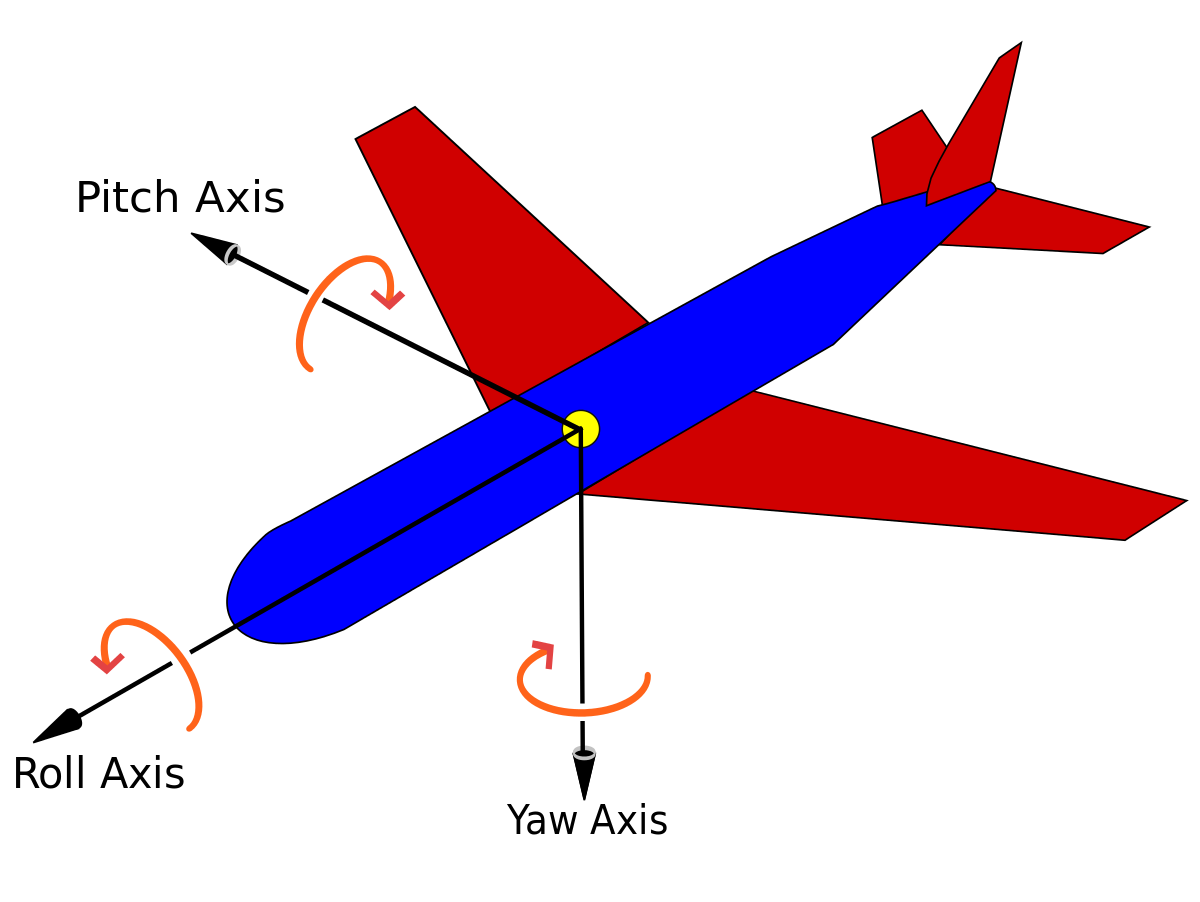
\includegraphics[width=0.6\textwidth]{euler_axes.png}
    \caption{Rozkład kątów Eulera}
    \label{fig:axes}
    % \vspace{0.5cm}
\end{figure}

Pitch to kąt, który obrazuje, jak bardzo patrzymy w górę lub w dół. Yaw reprezentuje wielkość tego jak bardzo patrzymy w lewo lub w prawo. Roll oznacza, jak bardzo się turlamy, co jest najczęściej używane w statkach kosmicznych i powietrznych. Każdy z kątów Eulera jest reprezentowany przez pojedynczą wartość, a za pomocą kombinacji wszystkich trzech z nich możemy obliczyć dowolny wektor rotacji w 3D.

W naszy systemie wykorzystaliśmy tylko kąty \textit{pitch} i \textit{yaw}, a do ich modyfikacji wykorzystujemy ruch myszki.


\subsection{Utworzenie podłoża}
Pierwszą rzeczą jaką postanowiliśmy utworzyć w naszym programie było podłoże na którym będzie stał nasz obiekt. 
\begin{cppcode}

void Floor::render(Camera camera, glm::mat4 projection, GLuint uniformProjection, GLuint uniformView, GLuint uniformModel)
{
	glm::mat4 model(1.0f);
	model = glm::mat4(1.0f);
	model = glm::translate(model, glm::vec3(0.0, -0.35f, 0.0f));
	glUniformMatrix4fv(uniformProjection, 1, GL_FALSE, glm::value_ptr(projection));
	glUniformMatrix4fv(uniformView, 1, GL_FALSE, glm::value_ptr(camera.ComputeCameraMatrix()));
	glUniformMatrix4fv(uniformModel, 1, GL_FALSE, glm::value_ptr(model));
}
\end{cppcode}

Podłoga została stworzona bez żadnego problemu, ale nie posiada żandej tekstury przez co jest niewidoczna. W celu dodania tekstury do obeikty wymagane było stworzenie meshu oraz funkcji odpowiedzialnych za ładowanie tekstur oraz przydzielanie ich do obiektów. Podczas realizacji projektu został wybrany mesh po to, aby w łątwiejszy sposób można było dodać teksturę do obeiktu jaki właśnie stworzyliśmy.Kod po wprowadzonych zmianach zyskał następujące rzeczy:
\begin{cppcode}
Floor::Floor(GLfloat size)
{
	unsigned int floorIndices[] = {
		0,2,1,
		1,2,3
	};

	GLfloat floorVertices[] = {
		-size,  0.0f, -size,   0.0f,  0.0f,   0.0f,  0.0f,  0.0f,
		 size,  0.0f, -size,  size,  0.0f,	0.0f,  0.0f,  0.0f,
		-size,  0.0f,  size,   0.0f,  size,	0.0f,  0.0f,  0.0f,
		 size,  0.0f,  size,  size,  size,  0.0f,  0.0f,  0.0f
	};

	mesh.CreateMesh(floorVertices, floorIndices, 32, 6);

	texture.LoadTextureA();
}

void Floor::render(Camera camera, glm::mat4 projection, GLuint uniformProjection, GLuint uniformView, GLuint uniformModel)
{
    ...
    
	texture.UseTexture();
	mesh.RenderMesh();
}
\end{cppcode}

Należy pamiętać również o tym, że jeżeli podłoga ma się pojawić w naszym programie to musi zostać dodana do głównej pętli programu.
\begin{cppcode}
    ...
	Floor floor(20.0f);
    ...
	while (!mainWindow.getShouldClose())
	{
    ...

		floor.render(camera, projection, uniformProjection, uniformView, uniformModel);
	...
	}
\end{cppcode}
%%%%%%%%%%%%%%%%%%%%%%%%%%%%%%%%%%%%%%%%%%%%%%%%%%%%%%%%%%%%%%%%%%%%%%%%%%%%%%%%%%%%%%%%%%%%%%%%%%%%%%%%%%

\subsection{Teksturowanie}
Każdy obiekt stworzony w naszym programie posiada własną teksturę. W tym celu została stworozny cały odrępny plik pod nazwą Texture.cpp. Posiada on funkcje ładowania tekstury z pliku jak i jej czysczenie. W celu przypisania przygotowanej tekstury do obeiktu wykorzystywana jest funkcja UseTexture, która podmienia aktualną teksturę obiektu na tą zadaną.
\begin{cppcode}

bool Texture::LoadTexture()
{
	unsigned char *texData = stbi_load(fileLocation, &width, &height, &bitDepth, 0);
	if (!texData)
	{
		printf("Failed to fint: %s\n", fileLocation);
		return false;
	}

	glGenTextures(1, &textureID);
	glBindTexture(GL_TEXTURE_2D,textureID);

	glTexParameteri(GL_TEXTURE_2D, GL_TEXTURE_WRAP_S, GL_REPEAT);
	glTexParameteri(GL_TEXTURE_2D, GL_TEXTURE_WRAP_T, GL_REPEAT);
	glTexParameteri(GL_TEXTURE_2D, GL_TEXTURE_MIN_FILTER, GL_LINEAR);
	glTexParameteri(GL_TEXTURE_2D, GL_TEXTURE_MAG_FILTER, GL_LINEAR);

	glTexImage2D(GL_TEXTURE_2D, 0, GL_RGB, width, height, 0, GL_RGB, GL_UNSIGNED_BYTE, texData);
	glGenerateMipmap(GL_TEXTURE_2D);

	glBindTexture(GL_TEXTURE_2D, 0);

	stbi_image_free(texData);

	return true;
}
bool Texture::LoadTextureA()
{
    ...
}
void Texture::UseTexture()
{
	glActiveTexture(GL_TEXTURE0);
	glBindTexture(GL_TEXTURE_2D, textureID);
}

void Texture::ClearTexture()
{
	glDeleteTextures(1, &textureID);
	textureID = 0;
	width = 0;
	height = 0;
	bitDepth = 0;
	fileLocation = "";

}

\end{cppcode}

Klasa posiada dwa typy funkcji LoadTexture, różnica polega na tym, że funkcja LoadTextureA posiada kanał alpha w teksturze. Aby dodać taką funkcjonalnośc do programu należało zmienić jedną linijkę kodu z:

\begin{cppcode}
	glTexImage2D(GL_TEXTURE_2D, 0, GL_RGB, width, height, 0, GL_RGB, GL_UNSIGNED_BYTE, texData);
\end{cppcode}
Na
\begin{cppcode}
	glTexImage2D(GL_TEXTURE_2D, 0, GL_RGBA, width, height, 0, GL_RGBA, GL_UNSIGNED_BYTE, texData);
\end{cppcode}
%%%%%%%%%%%%%%%%%%%%%%%%%%%%%%%%%%%%%%%%%%%%%%%%%%%%%%%%%%%%%%%%%%%%%%%%%%%%%%%%%%%%%%%%%%%%%%%%%%%%%%%%%%
\subsection{Stworzenie modeli 3D}

Tak jak to było wspomnianne we wstępie do dokumentacji, cały samochód został wykonany za pomocą programu Blender. Na początku jednak samochód był tworzony ręcznie, za pomocą trójkątów. Taki sposób tworzenia samochodu był bardzo pracochłonny oraz generował bardzo duże trudności podczas dodawania kolejnych elmentów auta, dlatego też autorzy zdecydowali się na utworzenie modelów w programie Blender, a następnie wyeksportowanie do takeigo formatu, aby nie było porblemu z ich implementacją w kodzie. 
Na samymm początku było tworzone podwozie pojazdu.

\begin{figure}[H]
    \centering
    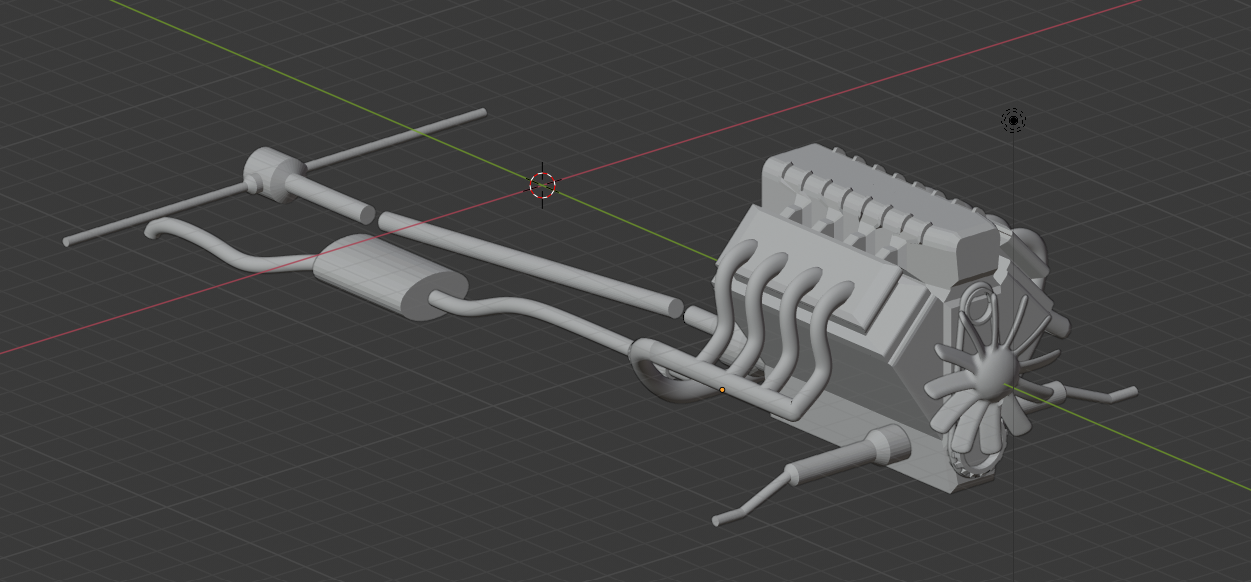
\includegraphics[width=\textwidth]{podwozie.png}
    \caption{Podwozie samochodu}
    \label{fig:podwozie}
    % \vspace{0.5cm}
\end{figure}

Jak widać na rysunku \ref{fig:podwozie} podwozie składa się z kilku  prostych elementów. Na samym początku znajduje się silnik wraz z przegubami, następnie wał kardana wędruje do tylnej osi. Poswtał również cały ukłąd wydechowy w samochodzie. Model ten nie posiada samych krzyżaków na wale, a także kół, gdyż aby te elementy były możliwe do zaanimowania musiały być tworzone jako osobne elementy. 

\begin{figure}[h!]
    \centering
    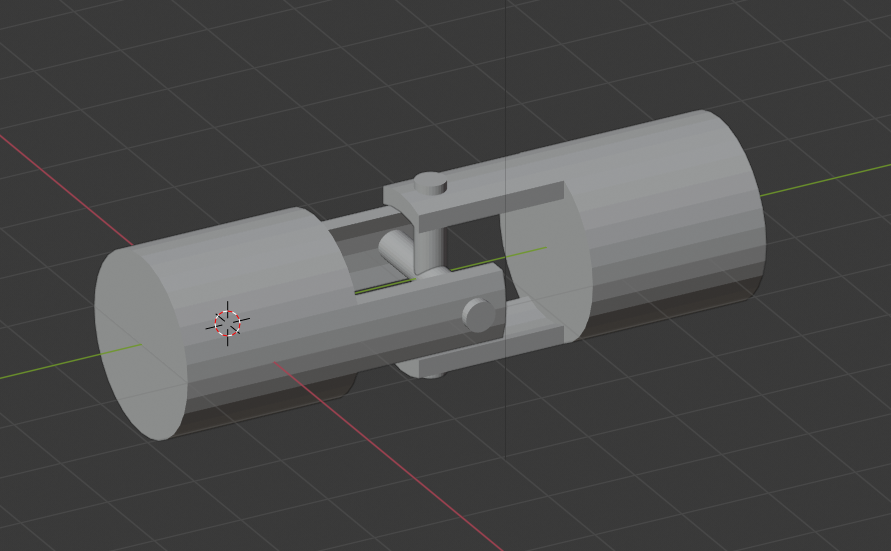
\includegraphics[width=\textwidth]{joint.png}
    \caption{Przegub Cardana}
    \label{fig:joint}
\end{figure}

 Na rysunku \ref{fig:joint} został zaprezentowany przegub Cardana, który jest istotnym elementem każdego wału napędowego w samochodzie. Przeguby w układach napędowych służą do przekazywania momentu obrotowego z jednego wału na inny, gdy osie obrotu tych wałów są do siebie nachylone. Stworzenie takeigo elementu w programie Blender nie było trudne. Taki przegub składa się z dwóch rzeczy: krzyżaka oraz jego uchwytu.

\begin{figure}[H]
    \centering
    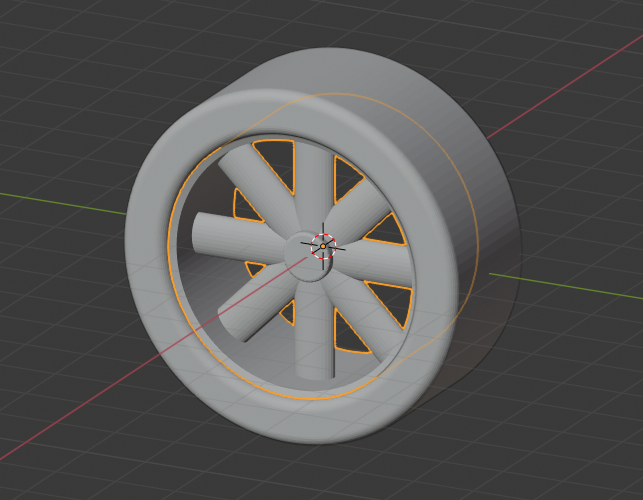
\includegraphics[width=\textwidth]{kolo.png}
    \caption{Koło samochodu}
    \label{fig:kolo}
\end{figure}
 
 W podobny sposób zostały wykonane koła dla samochodu. Zostało stworzone jedno koło, które następnie zostało wielokrotnie wykorzystane w procesie implementacji modelu. 

 \begin{figure}[h!]
    \centering
    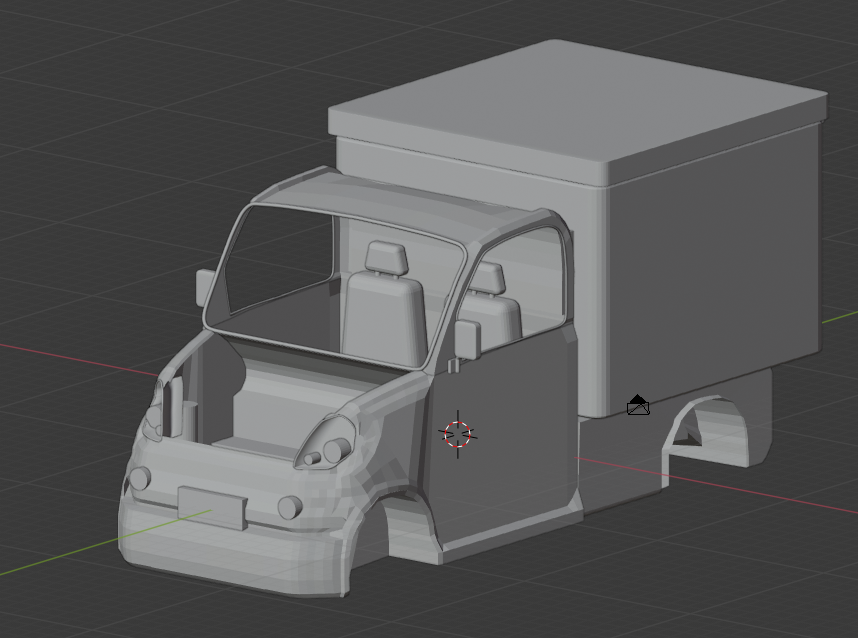
\includegraphics[width=\textwidth]{nadwozie.png}
    \caption{Nadwozie samochodu}
    \label{fig:nadwozie}
\end{figure}

Cała karoseria pojazdu na początku została stworzona jako jednolita bryła, niestety w taki sposób nie istnieje łatwy sposób na zaanimowanie pewnych części karoserii. Jako osobne obiekty zostały wyeksportowane takie lementy jak: maska oraz klapa bagażnika. W ten o to sposób samochód zyskał możliwość otwierania oraz zamykania klaby bagażnika oraz maski. 

\begin{figure}[H]
    \centering
    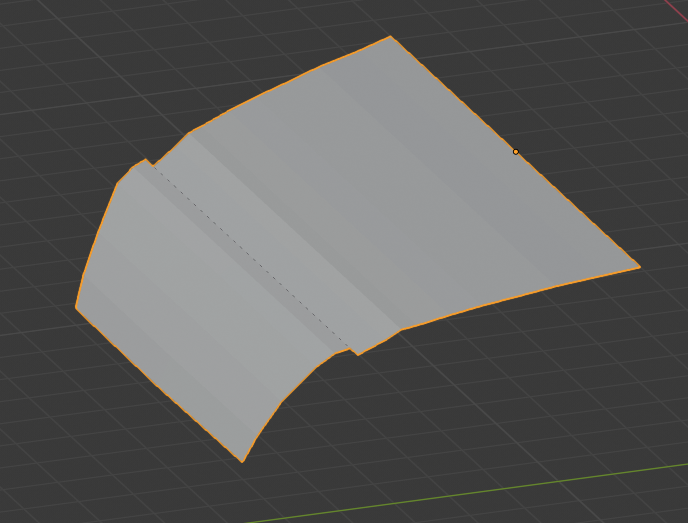
\includegraphics[width=\textwidth]{maska.png}
    \caption{Maska pojazdu}
    \label{fig:maska}
\end{figure}


%%%%%%%%%%%%%%%%%%%%%%%%%%%%%%%%%%%%%%%%%%%%%%%%%%%%%%%%%%%%%%%%%%%%%%%%%%%%%%%%%%%%%%%%%%%%%%%%%%%%%%%%%%
\subsection{Implementacja modeli w programie}
Stworzone w Blenderze modele 3D należało następnie dodać do projektu. Aby to zrobić posłużyliśmy się biblioteką \textit{Assimp}. Służy ona do importowania modeli 3D w różnych formatach do OpenGL'a.

Na początku utworzyliśmy klasę \mintinline{cpp}{Model}, która będzie służyła jako kontener na meshe, materiały i tekstury naszych obiektów. Klasa ta posiada kilka metod do ładowania poszczególnych części modelu, a także funkcję \mintinline{cpp}{RenderModel()}, dzięki której cały model jest renderowany w oknie.

\begin{figure}[H]
\begin{cppcode}
void Model::LoadModel(const std::string& fileName)
{
	Assimp::Importer importer;
	const aiScene *scene = importer.ReadFile(fileName, aiProcess_Triangulate | aiProcess_FlipUVs | aiProcess_GenSmoothNormals | aiProcess_JoinIdenticalVertices);
	LoadNode(scene->mRootNode, scene);
	LoadMaterials(scene);
}
\end{cppcode}
\caption{Funkcja ładująca model}
\end{figure}

\begin{figure}[H]
\begin{cppcode}
void Model::RenderModel()
{
	for (size_t i = 0; i < meshList.size(); i++) {
		unsigned int materialIndex = meshToTex[i];

		if (materialIndex < textureList.size() && textureList[materialIndex]) {
			textureList[materialIndex]->UseTexture();
		}
		meshList[i]->RenderMesh();
	}
}
\end{cppcode}
\caption{Funkcja renderująca model}
\end{figure}


%%%%%%%%%%%%%%%%%%%%%%%%%%%%%%%%%%%%%%%%%%%%%%%%%%%%%%%%%%%%%%%%%%%%%%%%%%%%%%%%%%%%%%%%%%%%%%%%%%%%%%%%%%

\subsection{Ożywienie samochodu}

W celu łatwiejszego zarządzania pojazdem utworzona została klasa \mintinline{cpp}{Car}, w której zawarte zostały najważniejsze parametry pojazdu. Funkcja \mintinline{cpp}{computeMovement()} służy do obliczenia pozycji samochodu oraz obrotu kół.

\begin{cppcode}
void Car::computeMovement(GLfloat deltaTime)
{
	GLfloat angle = (velocity * deltaTime) / 1.0f;
	wheelRotation += glm::degrees(angle);
	wheelRotation = fmod(wheelRotation, 360.0f);

	GLfloat roadLength = (velocity * deltaTime);
	position[0] += roadLength * sin(glm::radians(azymuth * 0.5));
	position[1] += roadLength * cos(glm::radians(azymuth * 0.5));
}
\end{cppcode}

Obliczane w tej funkcji parametry są potem uwzględniane przy renderowaniu modelu.

\begin{itemize}
\item Strzałka w górę — zwiększa prędkość pojazdu
\item Strzałka w dół — zmniejsza prędkość pojazdu
\item Strzałka w lewo — obrót kół w lewo
\item Strzałka w prawo — obrót kół w prawo

\item Klawisz 1 — otwieranie maski
\item Klawisz 2 — zamykanie maski
\item Klawisz 3 — otwieranie bagażnika
\item Klawisz 4 — zamykanie bagażnika
\end{itemize}

W funkcji \mintinline{cpp}{reactToInput()} modyfikowane są parametry samochodu w zależności od wciśniętych klawiszy. Dzięki temu doszła możliwość otwierania bagażnika oraz maski, a także skręcania kołami.

\begin{cppcode}
void Car::reactToInput(bool* keys)
{
	if (keys[GLFW_KEY_UP] && velocity < maxSpeed) velocity += 0.1f;
	if (keys[GLFW_KEY_DOWN] && velocity > -maxSpeed) velocity -= 0.1f;
	if (keys[GLFW_KEY_SPACE]) velocity = 0.0f;

	if (keys[GLFW_KEY_1] && hoodDegree < 90.0f) hoodDegree += 1.0f;
	if (keys[GLFW_KEY_2] && hoodDegree > 0.0f) hoodDegree -= 1.0f;

	if (keys[GLFW_KEY_3] && flapDegree < 90.0f) flapDegree += 1.0f;
	if (keys[GLFW_KEY_4] && flapDegree > 0.0f) flapDegree -= 1.0f;

	if (keys[GLFW_KEY_LEFT] && turnAngle < 30.0f) turnAngle += 0.2f;
	if (keys[GLFW_KEY_RIGHT] && turnAngle > -30.0f) turnAngle -= 0.2f;

	hideBody = keys[GLFW_KEY_B];
}
\end{cppcode}

%%%%%%%%%%%%%%%%%%%%%%%%%%%%%%%%%%%%%%%%%%%%%%%%%%%%%%%%%%%%%%%%%%%%%%%%%%%%%%%%%%%%%%%%%%%%%%%%%%%%%%%%%%
\section{Obsługa programu}
\begin{figure}[H]
    \centering
    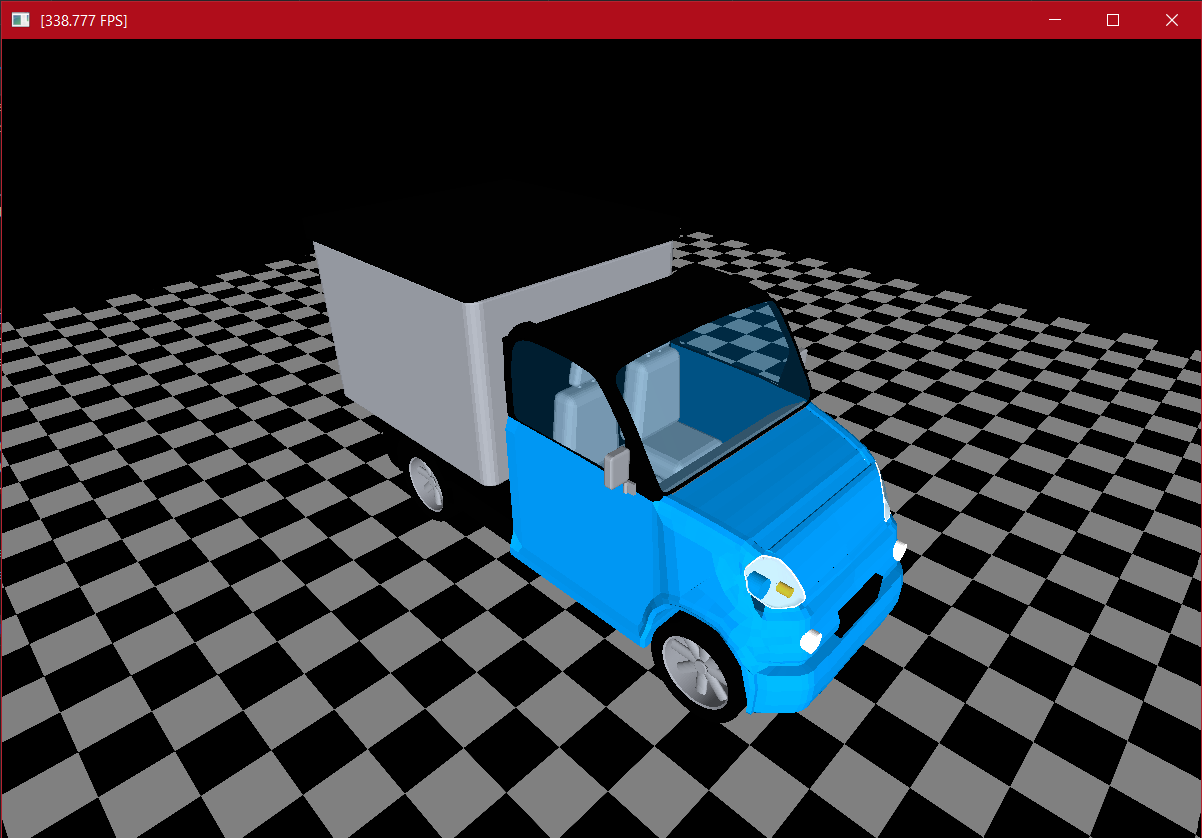
\includegraphics[width=\textwidth]{okno.png}
    \caption{Okno z samochodem}
    \label{fig:okno}
\end{figure}

\section{Podsumowanie}

Jak widać na rysunku \ref{fig:furgon} efekt naszej pracy jest bardzo bliski temu co staraliśmy się odwzorować. Nie był to łątwy projekt. Podczas jego realizacji napotkaliśmy wiele problemów. Niektóre z nich były łatwe w rozwiązaniu, np. problem z ruchem kamery oraz prawidłowym ładowaniu tekstur, a niektóre zajęły czasami tygodnie. Najtrudniejszym zadaniem okazało się poprawne umieszczenie stworzonego obiektu w Blenderze oraz jego zaanimowanie.

\begin{figure}[h!]
    \centering
    \subfloat{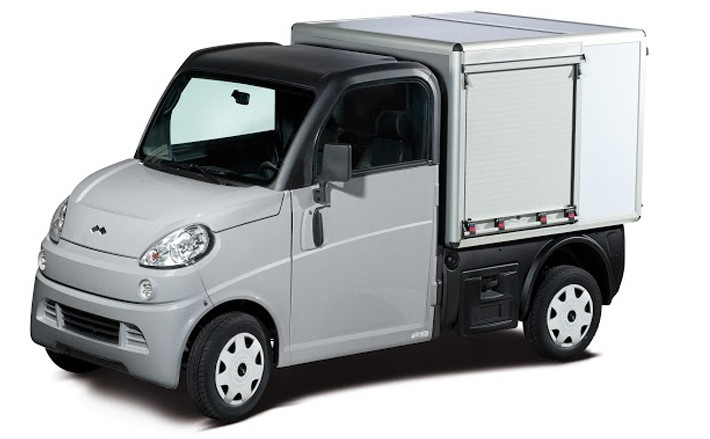
\includegraphics[width=0.5\textwidth]{furgon.jpg}}
    \subfloat{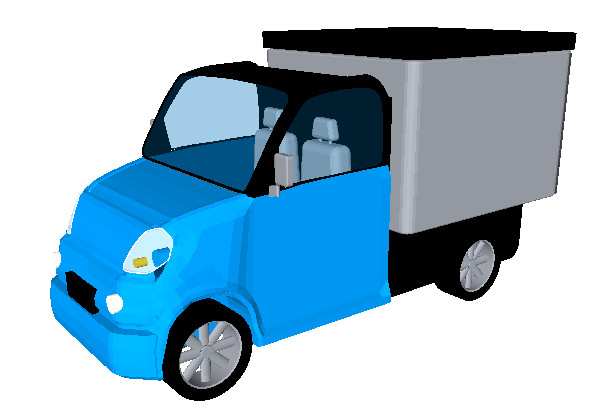
\includegraphics[width=0.5\textwidth]{gl_microcar.jpg}}
    \caption{Porównanie oryginału z utworzonym modelem}
    \label{fig:furgon}
    % \vspace{0.5cm}
\end{figure}

Autorzy projektu nigdy wcześniej nie mieli styczności z takim typem projektu. Wymagało to od nich nabycia zupełnie nowej wiedzy, aby zrealizować ten projekt bez problemów.

Podczas realizacji projektu niezwykle pomocnym okazały się wykłady prowadzone przez Pana Dr. Ryszarda Leniowskiego. Dzięki tym wykładą autorzy projektu mogli zrozumieć charakterysytkę projektu jaki sobie postawili za cel do zrealizowania, a także dogłębnie zorzumieć jak działają biblioteki graficzne.

% \begin{pythoncode}
% def forward(self, x):
%     y, sum_inputs = [x], []
%     for i in range(len(self.layers) + 1):
%         f = self.linear if i == len(self.layers) else self.activation
%         s = [np.dot(y[i], w) for w in self.weights[i]] + self.biases[i]
%         y.append(f(s))
%         sum_inputs.append(s)
%     return y, sum_inputs
% \end{pythoncode}


% \pagebreak
\begin{thebibliography}{9}
    \addcontentsline{toc}{section}{Literatura}
    \bibitem{zajdel_9} T. Gałaj, \emph{Learn OpenGL}, \href{https://shot511.github.io/pages/learnopengl/}{https://shot511.github.io/pages/learnopengl/}
\end{thebibliography}

\end{document}